\chapter{Метод роения частиц} \label{ParticleSwarmOptimisation}
\addcontentsline{toc}{chapter}{Метод роения частиц}    % Добавляем его в оглавление, если нет нумерации
\noindent
\emph{Метод роения частиц} (\emph{Particle Swarm Optimization}, PSO) является одним из алгоритмов коллективной оптимизации и основывается на имитации социального поведения в колонии живых организмов --- к примеру, стаи птиц или колонии муравьев, --- выполняющих коллективный поиск места с наилучшими условиями для существования. При поиске пищи каждая особь колонии передвигается по окружающей среде независимо от остальных организмов с некой долей случайности в своих движениях. Рано или поздно одна из особей находит пропитание и, будучи социальным организмом, сообщает об этом остальным, что стягивает ее соседей к данной пище.

\section{Алгоритм}
\noindent
Найдем глобальный экстремум функции~$F \colon \mathbb{R}^{n} \to \mathbb{R}$. Для определенности будем искать глобальный минимум:
\[
	F(x_i) \to \min \limits _{x_i \in \mathbb{R}^{n}}
\]

Пусть в нашем рое существует~$\ell$~частиц, тогда рой имеет вид~$x = \{x_i\}_{i = 1}^{\ell}, \ x_i \in U \subseteq \mathbb{R}^n$. Пусть также определен вектор скорости~$v = \{v_i\}_{i=1}^{\ell}$,~$i$-я компонента которого является скоростью~$i$-й частицы, $v_i \in U \subseteq \mathbb{R}^n$.

\begin{enumerate}
	\item Изначально случайным образом выбираем расположение роя $x(0)$ и скорость движения каждой частицы $v(0)$.

	\item Определяем новое расположение роя:
	\[
		x(t + 1) \equiv x(t) + v(t)
	\]

	\item Выбираем наилучшую точку для~$i$-й частицы:
	\begin{equation}
		\label{eq:personal_best}
		p_i(t)
		=
		\begin{cases}
			x_i(t),
			&
			F(x_i(t + 1)) \geq F(x_i(t))
			\\
			x_i(t + 1),
			&
			F(x_i(t + 1)) < F(x_i(t))
		\end{cases}, \ 1, ..., \ell
	\end{equation}

	Тогда вектор наилучших позиций для каждой частицы имеет вид:
	\[
		p(t) = \{p_i(t)\}_{i = 1}^{\ell}
	\]

	\item Выбираем наилучшую точку для всего сообщества:
	\begin{equation}
		\label{eq:social_best}
		g(t)
		\equiv
		\mathop{\mathrm{argmin}}_{i \in (1, ..., \ell)} \limits F(p_i(t))
	\end{equation}

	\item Обновляем скорость для~$i$-й частицы посредством следующей формулы:
	\begin{equation}
		\label{eq:new_velocity}
		v_i(t + 1)
		\equiv
		w
		v_i(t)
		+
		c_1
		\xi_1(t)
		[p_i(t) - x_i(t)]
		+
		c_2
		\xi_2(t)
		[g(t) - x_i(t)], \
		i = 1, ..., \ell
	\end{equation}

	где $w \in \mathbb{R}$ --- инерционный вес,~$c_1,\ c_2 \in \mathbb{R}$ --- коэффициенты ускорения, $\xi_1,\ \xi_2 \sim U(0, 1)$.

	Тогда векотр скорости имеет вид:
	\[
		v(t+1) = \{v_i(t + 1)\}_{i = 1}^{\ell}
	\]

	Три фактора влияют на частицу в положении $x_i(t)$. С одной стороны, когнитивное воздействие побуждает частицу двигаться к ее лучшей позиции $p_i(t)$, с другой стороны --- социальное воздействие побуждает частицу продвигаться в сторону лучшей позиции роя $g(t)$. Кроме того, собственная скорость $v_i(t)$ обеспечивает движение по инерции, что позволяет частице преодолевать локальные минимумы и исследовать неизвестные области заданного пространства. Таким образом, происходит переход от точки $x_i(t)$ в точку $x_i(t+1)$, что представлено на следующем графике:

	\vspace{10pt}

\begin{figure}[!h]
	\centering
	\tikzset{every picture/.style={line width=0.75pt}} %set default line width to 0.75pt

\begin{tikzpicture}[x=0.75pt,y=0.75pt,yscale=-1,xscale=1]
uncomment if require: \path (0,429); %set diagram left start at 0, and has height of 429

%Straight Lines [id:da4449765665231038]
\draw    (182.83,365.09) -- (182.83,155.34) ;
\draw [shift={(182.83,153.34)}, rotate = 450] [color={rgb, 255:red, 0; green, 0; blue, 0 }  ][line width=0.75]    (10.93,-4.9) .. controls (6.95,-2.3) and (3.31,-0.67) .. (0,0) .. controls (3.31,0.67) and (6.95,2.3) .. (10.93,4.9)   ;
%Straight Lines [id:da7153141724618748]
\draw [color={rgb, 255:red, 0; green, 0; blue, 0 }  ,draw opacity=1 ]   (182.83,365.09) -- (512.5,365.09) ;
\draw [shift={(514.5,365.09)}, rotate = 180] [color={rgb, 255:red, 0; green, 0; blue, 0 }  ,draw opacity=1 ][line width=0.75]    (10.93,-3.29) .. controls (6.95,-1.4) and (3.31,-0.3) .. (0,0) .. controls (3.31,0.3) and (6.95,1.4) .. (10.93,3.29)   ;
%Straight Lines [id:da049021320953235525]
\draw [color={rgb, 255:red, 0; green, 0; blue, 0 }  ,draw opacity=1 ]   (182.83,365.09) -- (58.11,247.89) ;
\draw [shift={(56.65,246.52)}, rotate = 403.22] [color={rgb, 255:red, 0; green, 0; blue, 0 }  ,draw opacity=1 ][line width=0.75]    (10.93,-3.29) .. controls (6.95,-1.4) and (3.31,-0.3) .. (0,0) .. controls (3.31,0.3) and (6.95,1.4) .. (10.93,3.29)   ;
%Straight Lines [id:da20232334639948002]
\draw [color={rgb, 255:red, 0; green, 0; blue, 0 }  ,draw opacity=1 ]   (182.83,365.09) -- (633.3,204.65) ;
\draw [shift={(635.19,203.98)}, rotate = 520.4] [color={rgb, 255:red, 0; green, 0; blue, 0 }  ,draw opacity=1 ][line width=0.75]    (10.93,-3.29) .. controls (6.95,-1.4) and (3.31,-0.3) .. (0,0) .. controls (3.31,0.3) and (6.95,1.4) .. (10.93,3.29)   ;
%Straight Lines [id:da30982294243702113]
\draw  [dash pattern={on 4.5pt off 4.5pt}]  (183.71,29.64) -- (479.85,30.9) ;
%Shape: Ellipse [id:dp3097132743634232]
\draw  [color={rgb, 255:red, 255; green, 255; blue, 255 }  ,draw opacity=1 ][fill={rgb, 255:red, 0; green, 0; blue, 0 }  ,fill opacity=1 ] (518.98,362.76) .. controls (518.98,357.83) and (522.93,353.85) .. (527.8,353.85) .. controls (532.66,353.85) and (536.61,357.83) .. (536.61,362.76) .. controls (536.61,367.68) and (532.66,371.66) .. (527.8,371.66) .. controls (522.93,371.66) and (518.98,367.68) .. (518.98,362.76) -- cycle ;
%Straight Lines [id:da6707373193501853]
\draw  [dash pattern={on 4.5pt off 4.5pt}]  (645.14,199.17) -- (514.24,63.27) -- (479.85,30.9) ;
%Shape: Ellipse [id:dp9920903593918595]
\draw  [color={rgb, 255:red, 255; green, 255; blue, 255 }  ,draw opacity=1 ][fill={rgb, 255:red, 0; green, 0; blue, 0 }  ,fill opacity=1 ] (40.39,240.61) .. controls (40.39,235.68) and (44.34,231.7) .. (49.2,231.7) .. controls (54.07,231.7) and (58.02,235.68) .. (58.02,240.61) .. controls (58.02,245.53) and (54.07,249.51) .. (49.2,249.51) .. controls (44.34,249.51) and (40.39,245.53) .. (40.39,240.61) -- cycle ;
%Shape: Ellipse [id:dp6112242856893209]
\draw  [color={rgb, 255:red, 255; green, 255; blue, 255 }  ,draw opacity=1 ][fill={rgb, 255:red, 0; green, 0; blue, 0 }  ,fill opacity=1 ] (174.02,365.09) .. controls (174.02,360.17) and (177.96,356.18) .. (182.83,356.18) .. controls (187.7,356.18) and (191.65,360.17) .. (191.65,365.09) .. controls (191.65,370.01) and (187.7,374) .. (182.83,374) .. controls (177.96,374) and (174.02,370.01) .. (174.02,365.09) -- cycle ;
%Shape: Ellipse [id:dp6835854741315035]
\draw  [color={rgb, 255:red, 255; green, 255; blue, 255 }  ,draw opacity=1 ][fill={rgb, 255:red, 0; green, 0; blue, 0 }  ,fill opacity=1 ] (636.32,199.17) .. controls (636.32,194.25) and (640.27,190.26) .. (645.14,190.26) .. controls (650.01,190.26) and (653.95,194.25) .. (653.95,199.17) .. controls (653.95,204.09) and (650.01,208.07) .. (645.14,208.07) .. controls (640.27,208.07) and (636.32,204.09) .. (636.32,199.17) -- cycle ;
%Straight Lines [id:da2902420192579651]
\draw  [dash pattern={on 4.5pt off 4.5pt}]  (182.83,148.74) -- (182.79,29.64) ;

% Text Node
\draw (143.08,220.88) node [anchor=north west][inner sep=0.75pt]  [font=\normalsize]  {$v_{i}( t)$};
% Text Node
\draw (375.46,269.9) node [anchor=north west][inner sep=0.75pt]  [font=\normalsize,rotate=-341.26,xslant=-0.03]  {$v_{i}( t+1)$};
% Text Node
\draw (183.03,324.8) node [anchor=north west][inner sep=0.75pt]  [font=\normalsize]  {$x_{i}( t)$};
% Text Node
\draw (609.4,209.67) node [anchor=north west][inner sep=0.75pt]  [font=\normalsize]  {$x_{i}( t+1)$};
% Text Node
\draw (511.93,326.66) node [anchor=north west][inner sep=0.75pt]  [font=\normalsize]  {$p_{i}( t)$};
% Text Node
\draw (62.39,222.19) node [anchor=north west][inner sep=0.75pt]  [font=\normalsize]  {$g( t)$};
% Text Node
\draw (271.18,48.68) node [anchor=north west][inner sep=0.75pt]  [font=\normalsize,rotate=-359.87,xslant=0]  {$c_{1} \xi _{1}( t)[ p_{i}( t) -x_{i}( t)]$};
% Text Node
\draw (385.65,117.39) node [anchor=north west][inner sep=0.75pt]  [font=\normalsize]  {$c_{2} \xi _{2}( t)[ g( t) -x_{i}( t)]$};
% Text Node
\draw (350.69,99.13) node [anchor=north west][inner sep=0.75pt]  [font=\normalsize] [align=left] {социальное воздействие};
% Text Node
\draw (252.05,31.73) node [anchor=north west][inner sep=0.75pt]  [font=\normalsize] [align=left] {когнитивное воздействие};
% Text Node
\draw (129.25,90.68) node [anchor=north west][inner sep=0.75pt]  [font=\normalsize]  {$wv_{i}( t)$};
% Text Node
\draw (110,73.14) node [anchor=north west][inner sep=0.75pt]  [font=\normalsize] [align=left] {инерция};
\end{tikzpicture}
\vspace{-30pt}
\caption{}
\end{figure}

	Алгоритм использует две последовательности равномерно распределенных случайных величин~$\xi_1(0), ..., \xi_1(t)$~и~$\xi_2(0), ..., \xi_2(t)$, которые масштабируются по константам~$c_1,\ c_2$. Данные константы влияют на максимальный размер шага, который частица может сделать за одну итерацию.	При~$c_1 = 0$~метод роения частиц будет опираться только на наилучшую позицию сообщества --- в таком случае алгоритм будет быстро сходиться, однако маловероятен факт нахождения глобального оптимума. При~$c_1 > 0$~метод использует связь всего сообщества --- скорость конвергенции падает, но глобальный оптимум оказывается более вероятным.

	\item Возвращаемся к 2 шагу, пока не достигнем оптимума.
\end{enumerate}

\section{Функция Розенброка}

\noindent
Функция Розенброка --- это невыпуклая функция вида
\[
	f(x, y) = (a - x)^2 + b(y-x^2)^2,
\]
использующаяся в качестве оценки производительности оптимизационных алоритмов. Она имеет глобальный минимум в точке $(a, a^2)$, где $f(a, a^2) = 0$.

\begin{figure}[ht]
	\centering
  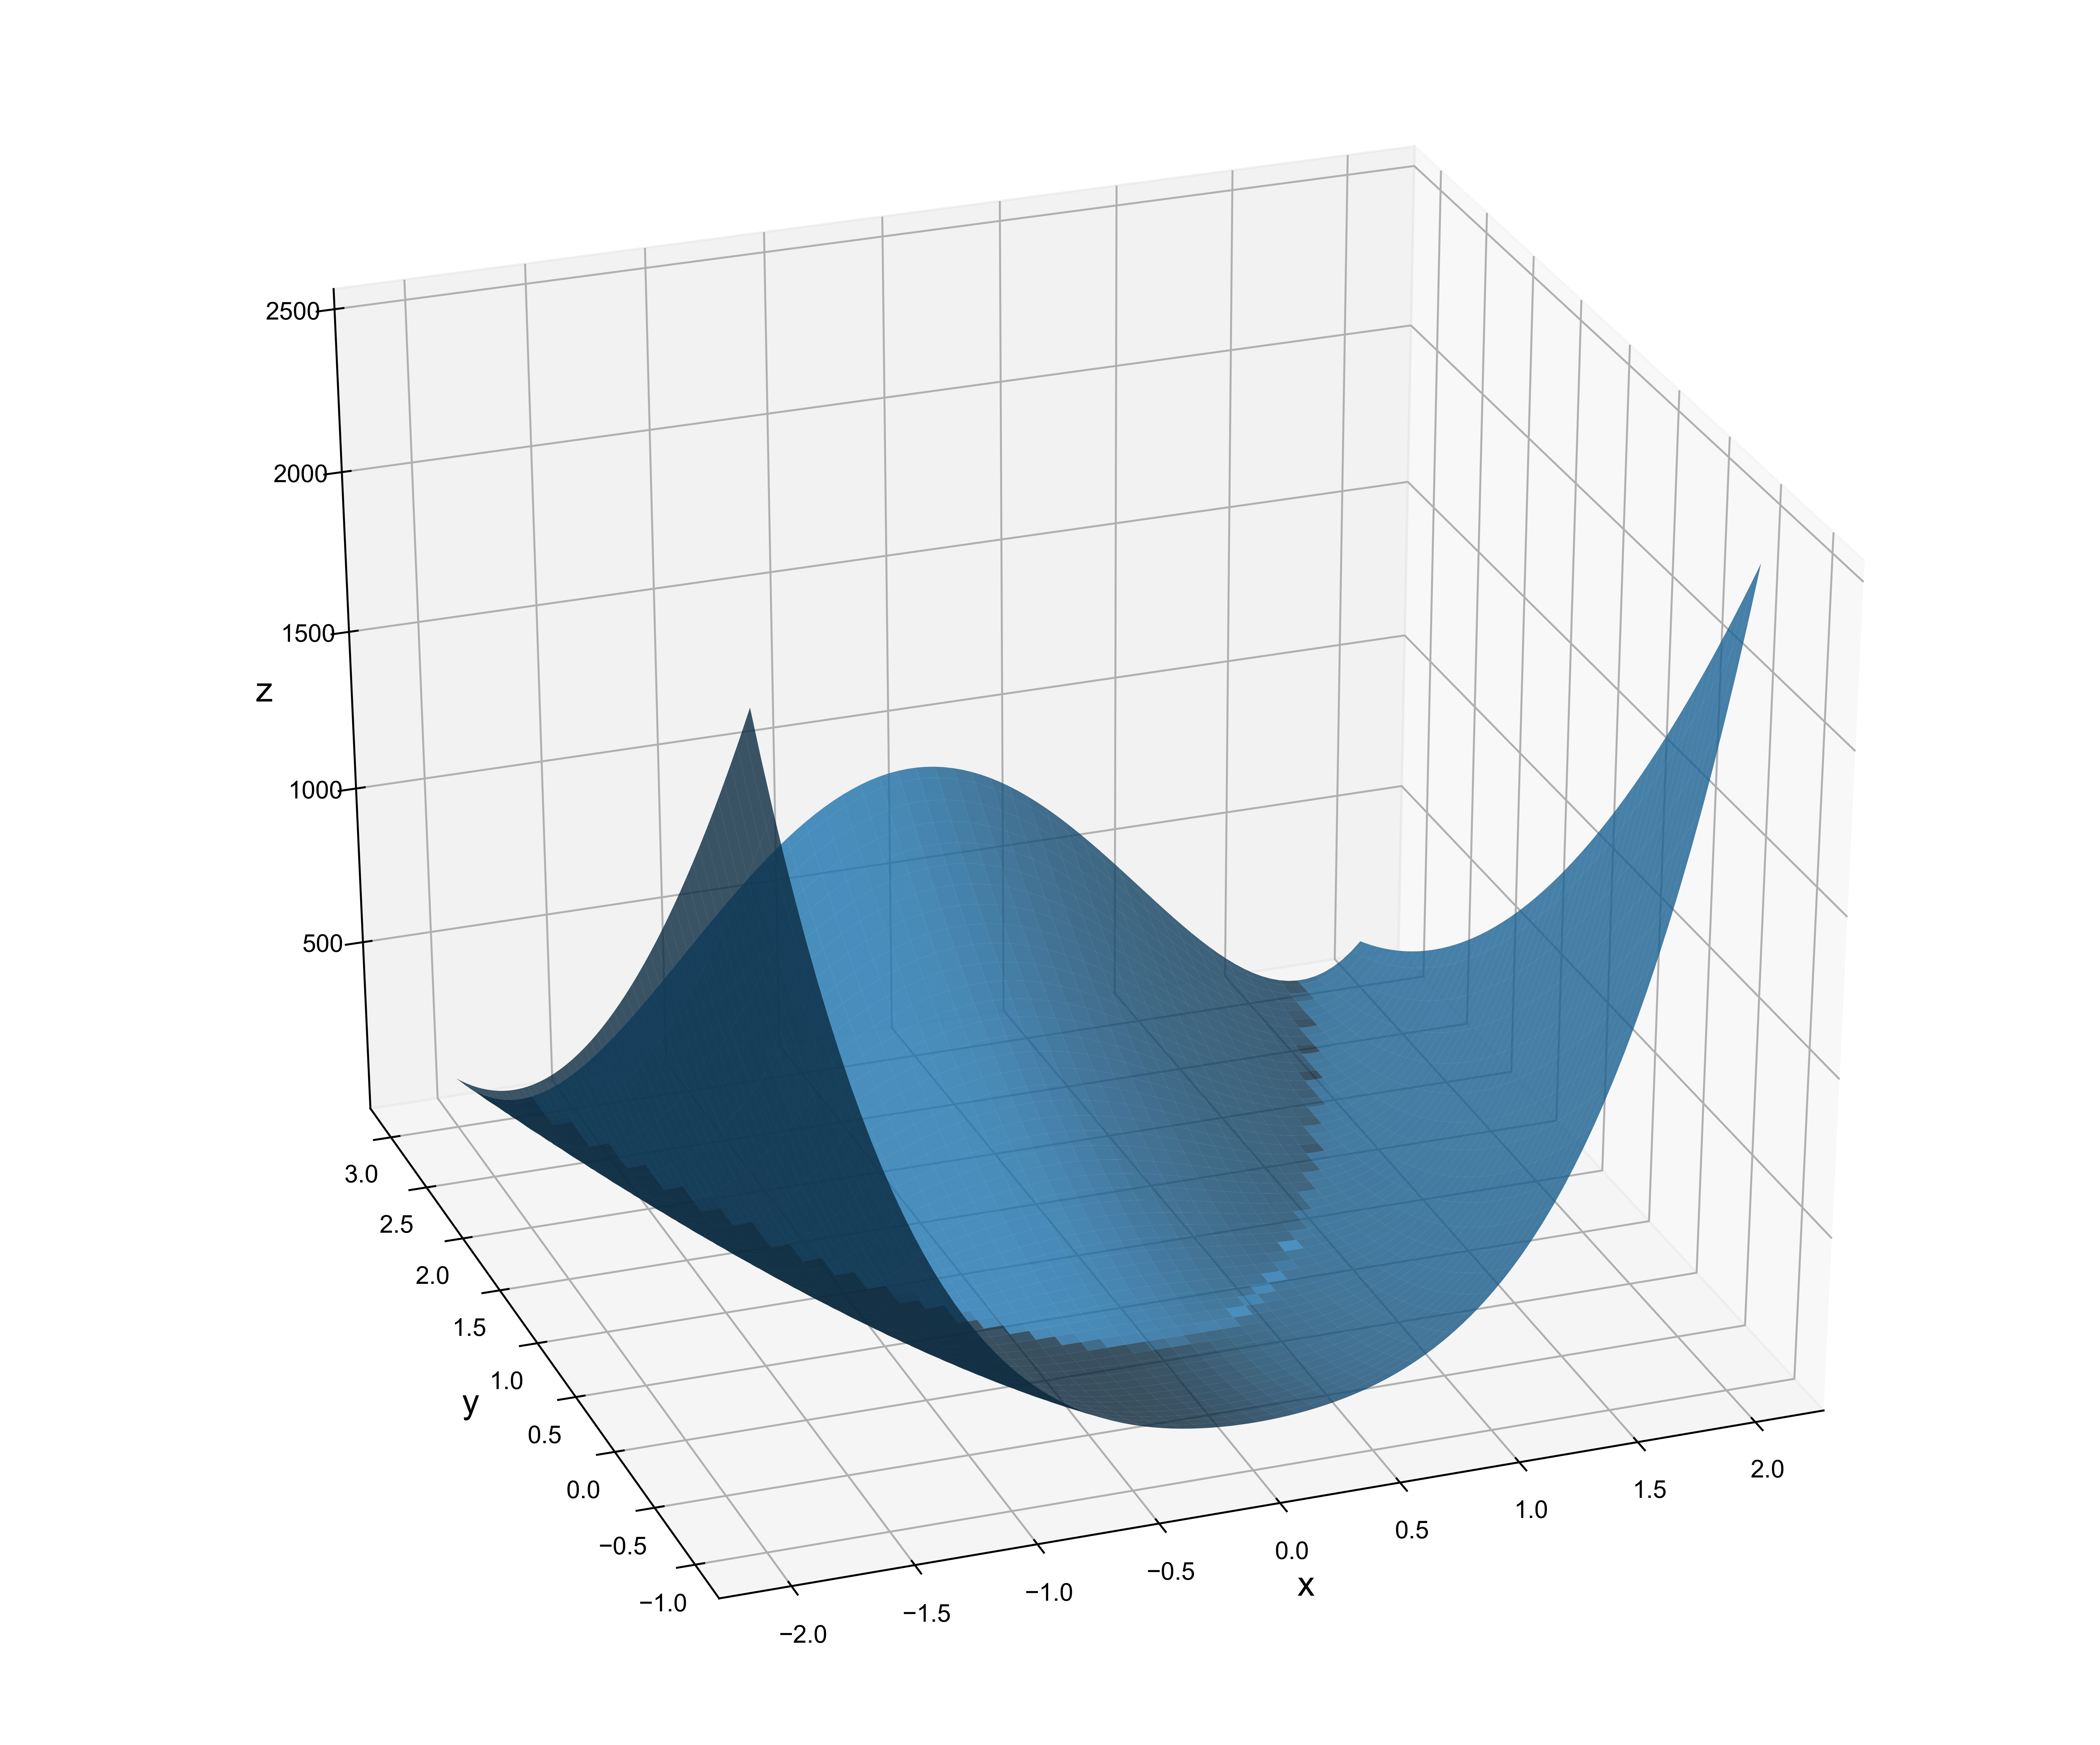
\includegraphics[width=\linewidth]{rosenbrock}
  \caption{ --- Функция Розенброка с параметрами $a = 1$, $b = 100$.}
  \label{img:rosenbrock}
\end{figure}


Обычно $a = 1$, $b=100$. Тогда функция Розенброка примет следующий вид (рис. \ref{img:rosenbrock}):
\[
	f(x, y) = (1 - x)^2 + 100(y-x^2)^2
\]

Глобальный минимум данной функции находится внутри <<долины>>: в нашем случае --- в точке $(1, 1)$. Найти долину достаточно легко, однако приблизиться к глобальному минимуму, считается, довольно сложно.

Только при $a = 0$, функция является симметричной, а ее минимум находится в начале координат.

Определим функцию Розенброка:
\begin{pyin}
def func(x):
  return (1 - x[0]) ** 2 + 100 * (x[1] - x[0] ** 2) ** 2
\end{pyin}

Инициализируем метод роения частиц, используя объектно-ориентированное программирование. В первую очередь cоздадим класс частиц.
\begin{pyin}
class Particle:
  def __init__(self, arg, space):
    self.pos = np.asarray([])      # расположение частицы
    self.velocity = np.asarray([]) # вектор скорости частицы
    self.pos_best = None           # лучшее расположение
    for i in range(arg):
       pos_i = np.random.uniform(space[i][0], space[i][1])
       self.pos = np.append(self.pos, pos_i)
       vel_i = np.random.uniform(0.2*space[i][0] , 0.2*space[i][1])
       self.velocity = np.append(self.velocity, vel_i)
    # pos_best --- это список, состоящий из лучшего расположения
    # частицы и значения функции в данной точке
    self.pos_best = [self.pos.copy(), func(self.pos)]

  def update_position(self):
    self.pos += self.velocity

  def update_velocity(self, w, c1, c2, swarm_best):
    inertion = w * self.velocity
    xi_1 = np.random.uniform()
    xi_2 = np.random.uniform()
    cognitive_acceler = c1 * xi_1 * (self.pos_best[0] - self.pos)
    social_acceler = c2 * xi_2 * (swarm_best - self.pos)
    self.velocity = inertion + cognitive_acceler + social_acceler

  def choose_personal_best(self):
    if func(self.pos) < func(self.pos_best[0]):
		   self.pos_best[0] = self.pos.copy()
		   self.pos_best[1] = func(self.pos)
\end{pyin}


Теперь cоздадим класс ParticleSwarmOptimisation. Поскольку инерционный вес $w$ должен быть близким к $1$, а коэффициенты ускорения $c_1$, $c_2$ должны быть достаточно малыми, при инициализации класса установим гиперпараметры по умолчанию равными следующим величинам: $w=1.0$, $c1=0.2$, $c2=0.2$. Посредством метода search\_global будем искать глобальный минимум функции Розенброка.

\begin{pyin}
class ParticleSwarmOptimisation:
  def __init__(self, ell=40, w=1.0, c1=0.2, c2=0.2, max_iter=1000,
	       tol=1e-6):
    """
    PARAMETERS:
    ell --- количество частиц в рое.
    w --- инерционный вес.
    c1 --- коэффициент ускорения когнитивного воздействия на частицу.
    c2 --- коэффициент ускорения социального воздействия на частицу.
    max_iter --- максимальное количество итераций.
    tol --- точность.
    """
    self.ell = ell
    self.w = w
    self.c1 = c1
    self.c2 = c2
    self.max_iter = max_iter
    self.tol = tol
    self.swarm_best = None # лучшее расположение для всего роя
    self.swarm = None      # расположение всех частиц (рой)

  def search_global(self, arg, space):
    """
    PARAMETERS:
    arg --- количество аргументов функции.
    space --- область поиска оптимума. Задается как список из
    кортежей, где кортеж --- это область значений
    одного аргумента функции.
    """
    self.arg = arg
    self.space = np.array(space)
    self.swarm = np.asarray([])

    # генерируем расположение роя
    for _ in range(self.ell):
       self.swarm = np.append(self.swarm,
                              Particle(self.arg, self.space))

    for k in range(self.max_iter):
\end{pyin}

\newpage
\begin{pyprint}
       for i in range(self.ell):
          # обновляем расположение частицы
          self.swarm[i].update_position()
          # сравниваем с лучшей точкой частицы
          self.swarm[i].choose_personal_best()

       # выбираем лучшую точку для роя
       if k != 0:
          dist_0 = self.dist(self.swarm_best[0])
          self.choose_social_best()
          dist_1 = self.dist(self.swarm_best[0])

          # останавливаем поиск в условиях заданной точности
          if (dist_0 != dist_1) and (abs(dist_0-dist_1) <= self.tol):
             break
       else:
          self.choose_social_best()

       # обновляем вектор скорости
       for i in range(self.ell):
          self.swarm[i].update_velocity(self.w, self.c1,
                                        self.c2, self.swarm_best[0])

    print(f"Глобальный оптимум: {self.swarm_best[0]}")
    print(f"Значение функции в данной точке: {self.swarm_best[1]}")

  def choose_social_best(self):
    best = min([[self.swarm[i].pos_best[0],
                 self.swarm[i].pos_best[1]] for i in range(self.ell)],
                 key=lambda x: x[1])
    self.swarm_best = best

  def dist(self, x):
    return np.sqrt(np.sum(x ** 2))
\end{pyprint}

Инициализируем рой c 100 частицами.
\begin{pyin}
sw = ParticleSwarmOptimisation(w=0.95, ell=100, tol=1e-20)
\end{pyin}

Найдем глобальный минимум. Перемещение роя в поисках глобального оптимума представлено на рисунке \ref{img:swarm}.
\begin{pyin}
np.random.seed(53)
sw.search_global(2, [(-10, 10),(-10, 10)])
\end{pyin}

\begin{pyout}
Глобальный оптимум: [1. 1.].
Значение функции в данной точке: 6.366439023928984e-22.
\end{pyout}

\begin{figure}[h!]
\centering
\includegraphics[width=\linewidth]{swarm}
\caption{ --- Расположение роя в разные моменты времени.}
\label{img:swarm}
\end{figure}

\begin{figure}[h!]
\centering
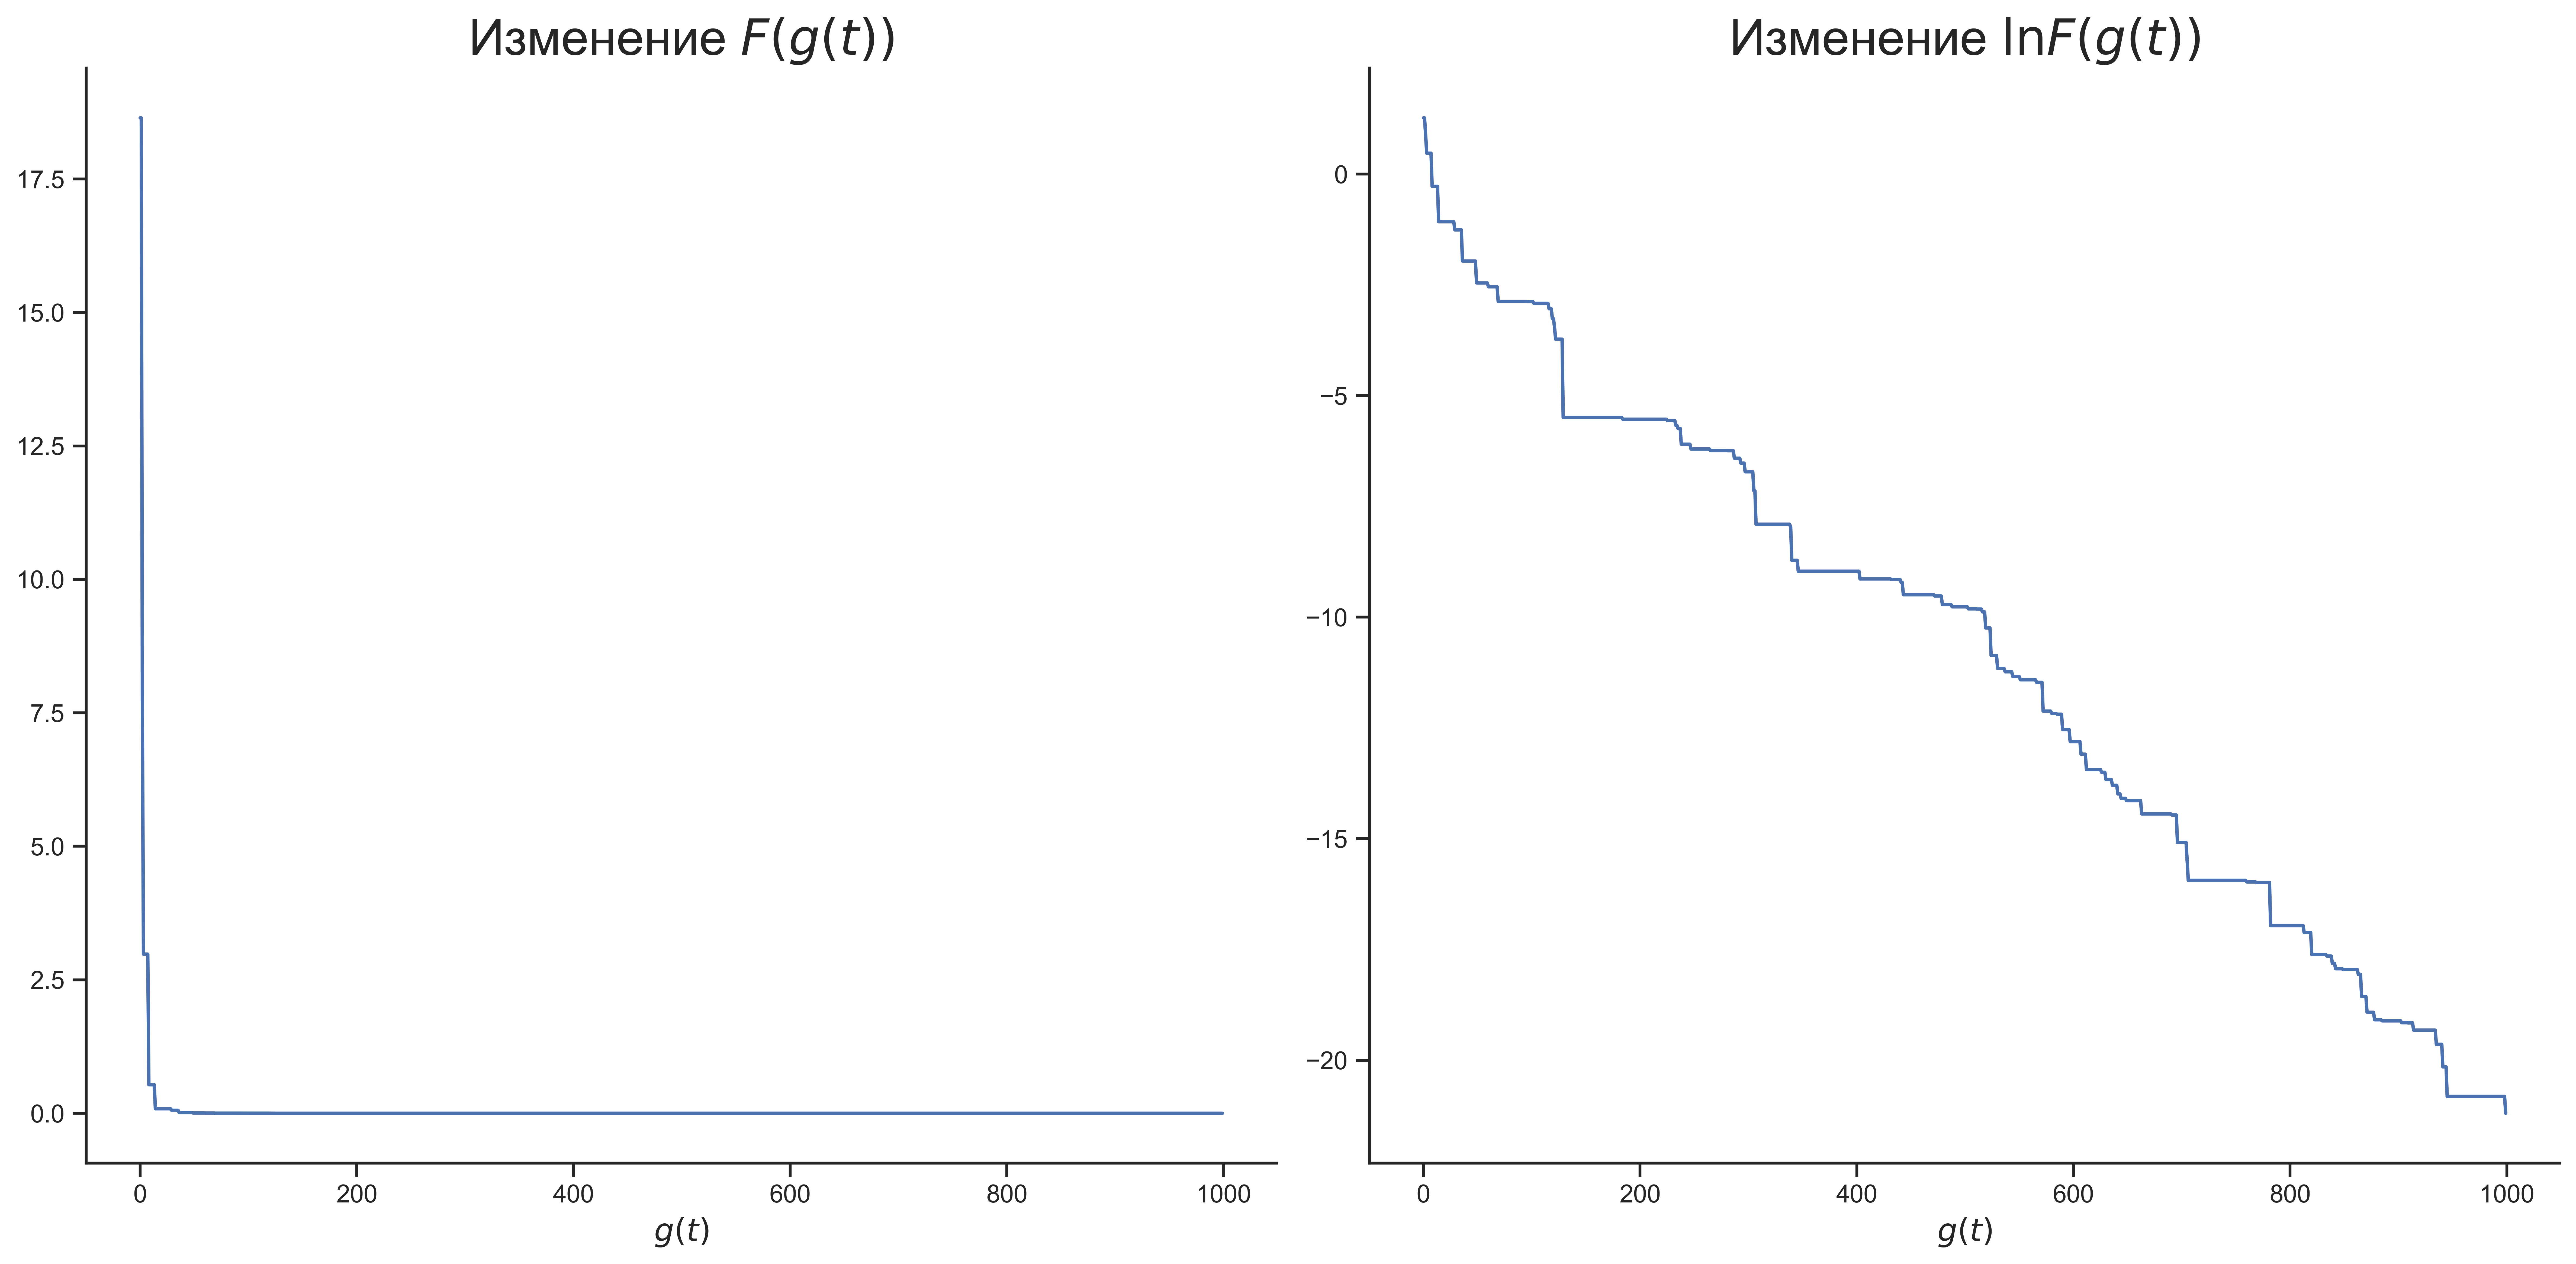
\includegraphics[width=\linewidth]{PSO}
\caption{ --- Оптимизационный процесс.}
\label{img:PSO}
\end{figure}

Из графиков на рисунке \ref{img:PSO} видно, что за 1000 итераций метод роения частиц сходится к глобальному минимуму функции Розенборока с экспоненциальной скоростью с точностью 6.37e-22. Средняя скорость реализации алгоритма составляет 1.79 секунды со стандартным отклонением в 0.111 секунд.
